\chapter{Experiment of Rivet-HSB hybrid Connection}
\label{ch3}

%%%%%%%%%%%%%%%%%%%%%%%%%%%%%%%%%%%%%%%
% IMPORTANT
\begin{spacing}{1.25} %THESE FOUR
\minitoc % LINES MUST APPEAR IN
\end{spacing} % EVERY
\onehalfspacing % CHAPTER
% COPY THEM IN ANY NEW CHAPTER
%%%%%%%%%%%%%%%%%%%%%%%%%%%%%%%%%%%%%%%

\section{Slip coefficient of riveted joint}

\subsection{background}

Rivets were widely used in the world to fasten steel members in the early days, and also used for cross-section connections for steel bridges. Since 1950, countries worldwide have been issued design specifications for high-strength bolts connection, and high-strength bolts connection have gradually replaced rivet connections. However, many riveted bridges are still in service \cite{Collette2014Experimental1880s1890s}. Some of the rivets might be corroded and loosen due to deterioration of the paint coating. The reduction of the volume of a rivet's head is severely affected fatigue life \cite{Heinemeyer2011TheConnections}. Studies have also pointed out the influence of rivets' material loss on these bridge structure elements' remaining bearing capacity \cite{Hashimoto2010,Macho2016}. For structural performance recovery or to extend their service life, the riveted bridges have to repair or reinforce by replacing the corroded rivets with high-strength bolts. Replacing the rivets with a high-strength bolt for changing to the frictional joint is a desirable approach to repairing the corroded riveted joint \cite{KOMATSU2015}. 
    
Applying such repair, whether it satisfies the frictional joints' performance requirements depends on the slip coefficient. However, the riveted joint surface's slip coefficient with red lead paint for corrosion is not specified. Therefore, giving a proper evaluation of the slip coefficient is one of the purposes of this paper.
Lead is an excellent anti-corrosive, lead-based paint that could be well protecting a steel structure from the element. Especially red lead (Pb3O4) was once widely used for bridges anti-corrosion paint. However, Lead-based paint has been a significant cause of lead poisoning. Countries around the world are beginning to call for an end to the use of Lead-based paint. The U.S. Consumer Product Safety Commission (CPSC) has already started banning lead-based paint in 1977 \cite{CPSC1977}. In 1987, Japan completely stopped using red lead as anti-corrosion paints for steel structures \cite{rtri1987Steel}. So far, the use of red lead has been completely discontinued and replaced by inorganic resin coatings. Red lead and rivets are used on steel bridges almost in the same period. Since rivets are designed to transmit load by shearing force, the friction performance of riveted joint surfaces with red lead paint is unspecified. 
In this study, the authors have got the opportunity to obtain a 90-year-old riveted bridge's cross-beam. The joint part was cut out from this bridge's cross-beam and evaluated the riveted joint surface's aging condition in natural corrosion weakening by microscope observation and elemental analysis. In addition, the slip test is conducted to investigate the joint surface's slip coefficient of the riveted joints experimentally. Finally, the pressure distribution test is conducted using a pressure measurement film to explore the pressure distribution and the effective contact pressure area of riveted joints' surface.


\subsection{Joint faying surface's aging condition}

The bridge of the research object has been in use for 90 years. The bridge's paint was probably damaged, and the joint surface was probably corroded due to aging. In order to investigate the condition of the aging bridge joint's surface, 40mm x 40mm compact specimens cut out from the joint to conduct microscope observation, Fourier-transform infrared spectroscopy analysis (FT-IR), and Energy Dispersive X-ray Spectroscopy (EDX) analysis.

\subsubsection{Microscope observation} \label{ch3sec2-1}

Depending on where the specimen was taken out, the red lead's aging condition has been found different. The research has shown that the red lead paint adjacent to the rivet hole has been compromised due to high temperature and clamping force by riveting. The friction coefficient may be affected by this \cite{Leonetti2020RivetBridges}.

The red lead on the joint surface has partly peeled off, and the black oxide of the steel can be observed, which indicates that the red lead's adhesion has become poor over aging, as shown in Fig. \ref{ch3fig2b}

\begin{figure}
    \centering
    \begin{subfigure}[t]{0.4\textwidth}
    \includegraphics[width=\linewidth]{imgs/ch3/fig2a.png}
    \caption{Normally}
    \label{ch3fig2a}  
    \end{subfigure}
    \hfill
    \begin{subfigure}[t]{0.4\textwidth}
    \includegraphics[width=\linewidth]{imgs/ch3/fig2b.png}
    \caption{Seriously}
    \label{ch3fig2b}  
    \end{subfigure}
    \caption{Faying surface for riveted joint}
\end{figure}

As shown in Fig. \ref{ch3fig3}, the joint surface was observed with an electron microscope of 50 times and 600 times. The orange-red substance is red lead, and the black primer is the black oxide of steel. No obvious traces of rust are found on the joint surface. The light reflecting material in the picture is a resin coating, and it will be confirmed by elemental analysis for the next section.

\begin{figure}
    \centering
    \begin{subfigure}[t]{0.4\textwidth}
    \includegraphics[width=\linewidth]{imgs/ch3/fig3a.jpeg}
    \caption{50X}
    \label{ch3fig3a}  
    \end{subfigure}
    \hfill
    \begin{subfigure}[t]{0.4\textwidth}
    \includegraphics[width=\linewidth]{imgs/ch3/fig3b.jpeg}
    \caption{600X}
    \label{ch3fig3b}  
    \end{subfigure}
    \caption{Microscope observation}
    \label{ch3fig3}
\end{figure}

\subsubsection{FT-IR and EDX analysis}

This study randomly selected three specimens from different positions of the joint and conducted FT-IR analysis on the joint surface. Furthermore, the presence of elements on the joint surface detected by EDX analysis. FT-IR spectra of the joint surface are illustrated in Fig. \ref{ch3fig4}. The spectrum consists of many sharp and weak bands in the region of 700–900 cm-1, in addition to a few bands in the region of 1,500–2,000 cm-1. Most of the main peaks corresponding to vinyl acetate (C4H6O2) were detected \cite{baskaran2004Vibrational}, but no main peaks corresponding to Iron (III) oxide (Fe2O3) were found. The study has shown that incorporating various metallic additives into polymer matrices can produce polymer-matrix composites and improve their properties for specific applications \cite{dong2006Polyvinylbutyral}. In order to enhance the adhesion of red lead, a resin-based primer is usually applied before the red lead. It can be considered that the vinyl acetate detected by FT-IR acts as a resin-based primer to enhance the adhesion of red lead.

\begin{figure}
    \centering
    \begin{minipage}[t]{0.7\textwidth}
    \includegraphics[width=\linewidth]{imgs/ch3/fig4.png}
    \caption{FT-IR spectra of the joint surface}
    \label{ch3fig4}  
    \end{minipage}
    \begin{minipage}[t]{0.7\textwidth}
    \includegraphics[width=\linewidth]{imgs/ch3/fig5.png}
    \caption{EDX-spectrum of the joint surface}
    \label{ch3fig5}  
    \end{minipage}
\end{figure}

From Fig. \ref{ch3fig5}, it can be inferred that the lead oxide on the joint surface was confirmed to exist on the joint surface, and there was also iron oxide. By means of FT-IR spectra that can confirm iron oxide is not red rust(iron(III) oxide), but a black oxide film formed when the steel is manufactured.


\subsection{Compact slip test}

\subsubsection{Loading and measuring methods}

Fig. \ref{ch3fig6} shows a loading machine and loading methodology, and Fig. \ref{ch3fig6a}, Fig. \ref{ch3fig6b} shows the general diagram and the detailed diagram, respectively. A screw-jack applies a horizontal load to two sets of specimens until it reaches the target clamping force. And they are then applying a vertical load to the specimens by a universal loading machine. There is a Displacement Transducer on each side of specimens, and they will be initialed to monitor the slip of the test specimen after the horizontal load is complete. Both horizontal and vertical loads applied were monitored by using a load cell.

\begin{figure}
    \centering
    \begin{subfigure}[t]{0.58\textwidth}
    \includegraphics[width=\linewidth]{imgs/ch3/fig6a.png}
    \caption{General diagram}
    \label{ch3fig6a}  
    \end{subfigure}
    \hfill
    \begin{subfigure}[t]{0.38\textwidth}
    \includegraphics[width=\linewidth]{imgs/ch3/fig6b.png}
    \caption{Detailed diagram}
    \label{ch3fig6b}  
    \end{subfigure}
    \caption{Test setup}
    \label{ch3fig6}
\end{figure}

The universal loading machine will be loading on 0.5 kN/s until a slip occurred. Then, the slip coefficient is calculated by the relationship between the vertical load and displacement.

\subsubsection{Specimens}

A total of 48 set specimens are cut out from the same riveted bridge's joint. The position of cut out and the size of specimens as shown in Figure 7a, and b respectively. In order to explore the influence of the clamping force on the slip coefficient, the specimens are divided into three groups according to the different clamping forces introduced. The three groups of specimens are 24 sets of 100\% standard clamping forces, 12 sets of 75\%, and 50\% standard clamping forces $N$. 

\begin{figure}
    \centering
    \begin{subfigure}[t]{0.48\textwidth}
    \includegraphics[width=\linewidth]{imgs/ch3/fig7a.png}
    \caption{Cross-beam}
    \label{ch3fig7a}  
    \end{subfigure}
    \hfill
    \begin{subfigure}[t]{0.48\textwidth}
    \includegraphics[width=\linewidth]{imgs/ch3/fig7b.png}
    \caption{Specimens section}
    \label{ch3fig7b}  
    \end{subfigure}
    \caption{Specimens' cut out location and size}
\end{figure}

The standard clamping force is calculated by multiplying the standard bolt contact pressure by the contact area. The assumed contact pressure area was calculated as the contact pressure distributed at 45° \cite{rotscher1927maschinenelemente}, as shown in Fig. \ref{ch3fig8}. When the splice plate's thickness is 12 mm, the standard bolt contact pressure can be calculated as 64.9 N/mm2. Here it is assumed that the bolt is the most commonly used F10T-M22 in Japanese bridges.


\begin{figure}
\centering
\includegraphics[width=0.65\linewidth]{imgs/ch3/fig8.pdf}
\caption{Definition of clamping area (unit: mm)}
\label{ch3fig8}  
\end{figure}

For example, for the M22 size bolt, the euivalent contact area $A_{ct-m22}$ is:
\begin{equation*}
    A_{ct-m22} = \pi (r_h-r_b)^2
\end{equation*}

Where, the  bolt shank radius $r_b$ is 11 mm, bolt hole radius $r_h$ is 11.75 mm.
the equivalent contact pressure $\sigma_{ct-m22}$ is:
\begin{equation*}
    \sigma_{ct-m22} = \frac{N}{A_{M22}} = 64.9 Mpa
\end{equation*}

Where, $N$ is the bolt standard preload, M22-F10T bolt is 205 kN.
The applied horizontal force (Converted preload) $N_{cp}$ is 
\begin{equation*}
    N_{cp} = \sigma_{ct-m22} \times A_{cts} =64.9 \times 40 \times 40 = 103.8 kN
\end{equation*}
Where, $A_{cts}$ is specimens size for compact slip test


\subsubsection{Test result}

The test results are summarized in Table \ref{ch3tab1}. The table summarizes the slip coefficients and their variation of all the specimens with 100\%, 75\%, and 50\% of standard clamping force.

\begin{table}[htbp]
\centering
\caption{Summary of the slip coefficient and estimation of variability}
\label{ch3tab1}
\scalebox{0.95}{
\begin{tabular}{@{}cccccccc@{}}
\toprule
\multirow{3}{*}{Specimens} &
  \multicolumn{3}{c}{Slip coefficient} &
  \multirow{3}{*}{\begin{tabular}[c]{@{}c@{}}Standard \\ Deviation \\ (SD, $\sigma$) \end{tabular}} &
  \multirow{3}{*}{\begin{tabular}[c]{@{}c@{}}Standard \\ Error \\ (SE) \end{tabular}} &
  \multirow{3}{*}{\begin{tabular}[c]{@{}c@{}}Coefficient \\ of Variation \\ (C.V.) \end{tabular}} &
  \multirow{3}{*}{\begin{tabular}[c]{@{}c@{}}The \\ Number \\ of data \end{tabular}} \\ \cmidrule(lr){2-4}
        & \multirow{2}{*}{Average} & \multirow{2}{*}{Max}   & \multirow{2}{*}{Min}   &        &        &        &    \\
        &   &     &     &        &        &        &    \\ \midrule
All     & 0.274   & 0.386 & 0.173 & 0.0525 & 0.0076 & 0.1917 & 48 \\
100\%CF & 0.291   & 0.386 & 0.192 & 0.0491 & 0.0100 & 0.1688 & 24 \\
75\%CF  & 0.240   & 0.341 & 0.173 & 0.0482 & 0.0139 & 0.2009 & 12 \\
50\%CF  & 0.274   & 0.351 & 0.208 & 0.0504 & 0.0145 & 0.1839 & 12 \\ \bottomrule
\end{tabular}}
\end{table}

The average slip coefficient is 0.274, the coefficient of variation is 0.19, and the -2σ is 0.169. It can be found that the degree of dispersion of the slip coefficient is not low. Furthermore, it could be concluded that the slip coefficient from the slip test follows a normal distribution by the Shapiro-Wilk normality test \cite{shapiro1965Analysis}. The normal distribution of the slip coefficient is shown in Fig. \ref{ch3fig10}. The 95\% confidence interval is presented as the arithmetic mean ± 1.96 SE (Standard Error) (0.259--0.289).

\begin{figure}
    \centering
    \begin{subfigure}[t]{0.48\textwidth}
    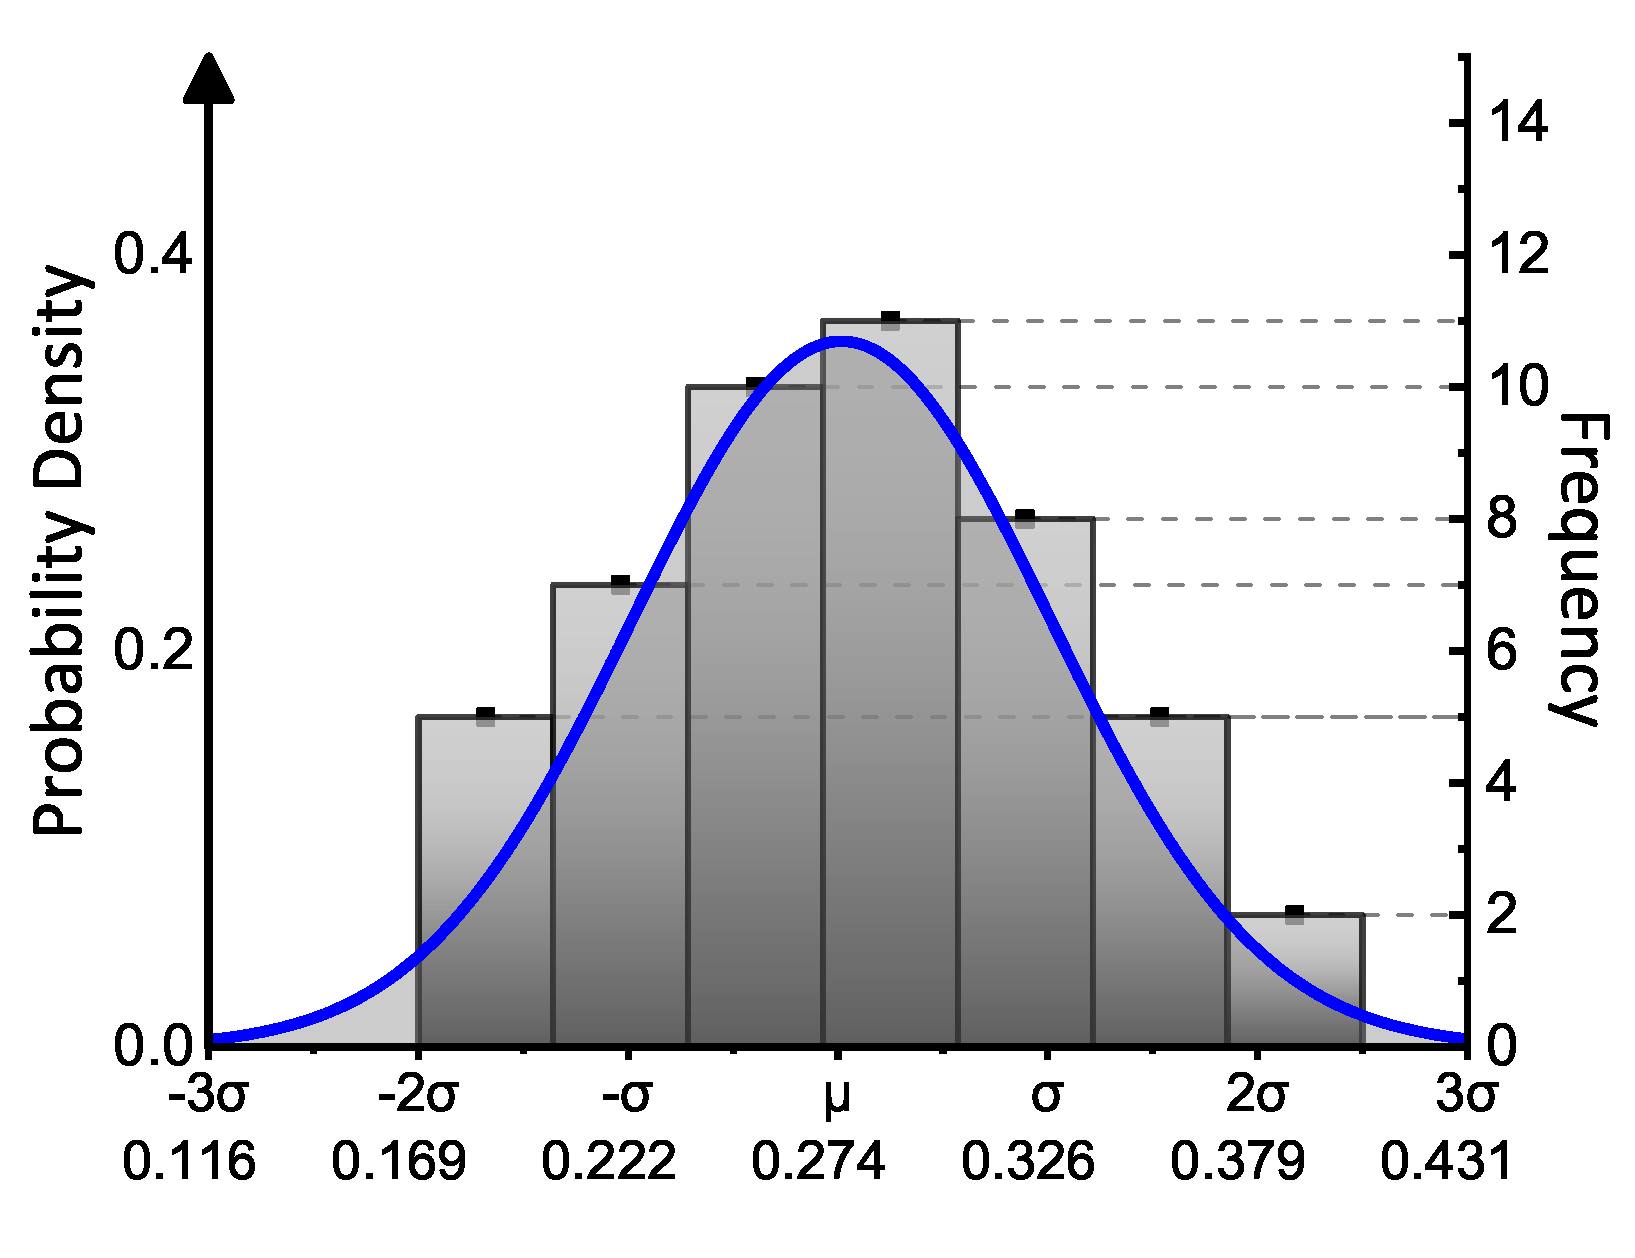
\includegraphics[width=\linewidth]{imgs/ch3/fig10a.eps}
    \caption{Normal distribution}
    \label{ch3fig10a}  
    \end{subfigure}
    \hfill
    \begin{subfigure}[t]{0.48\textwidth}
    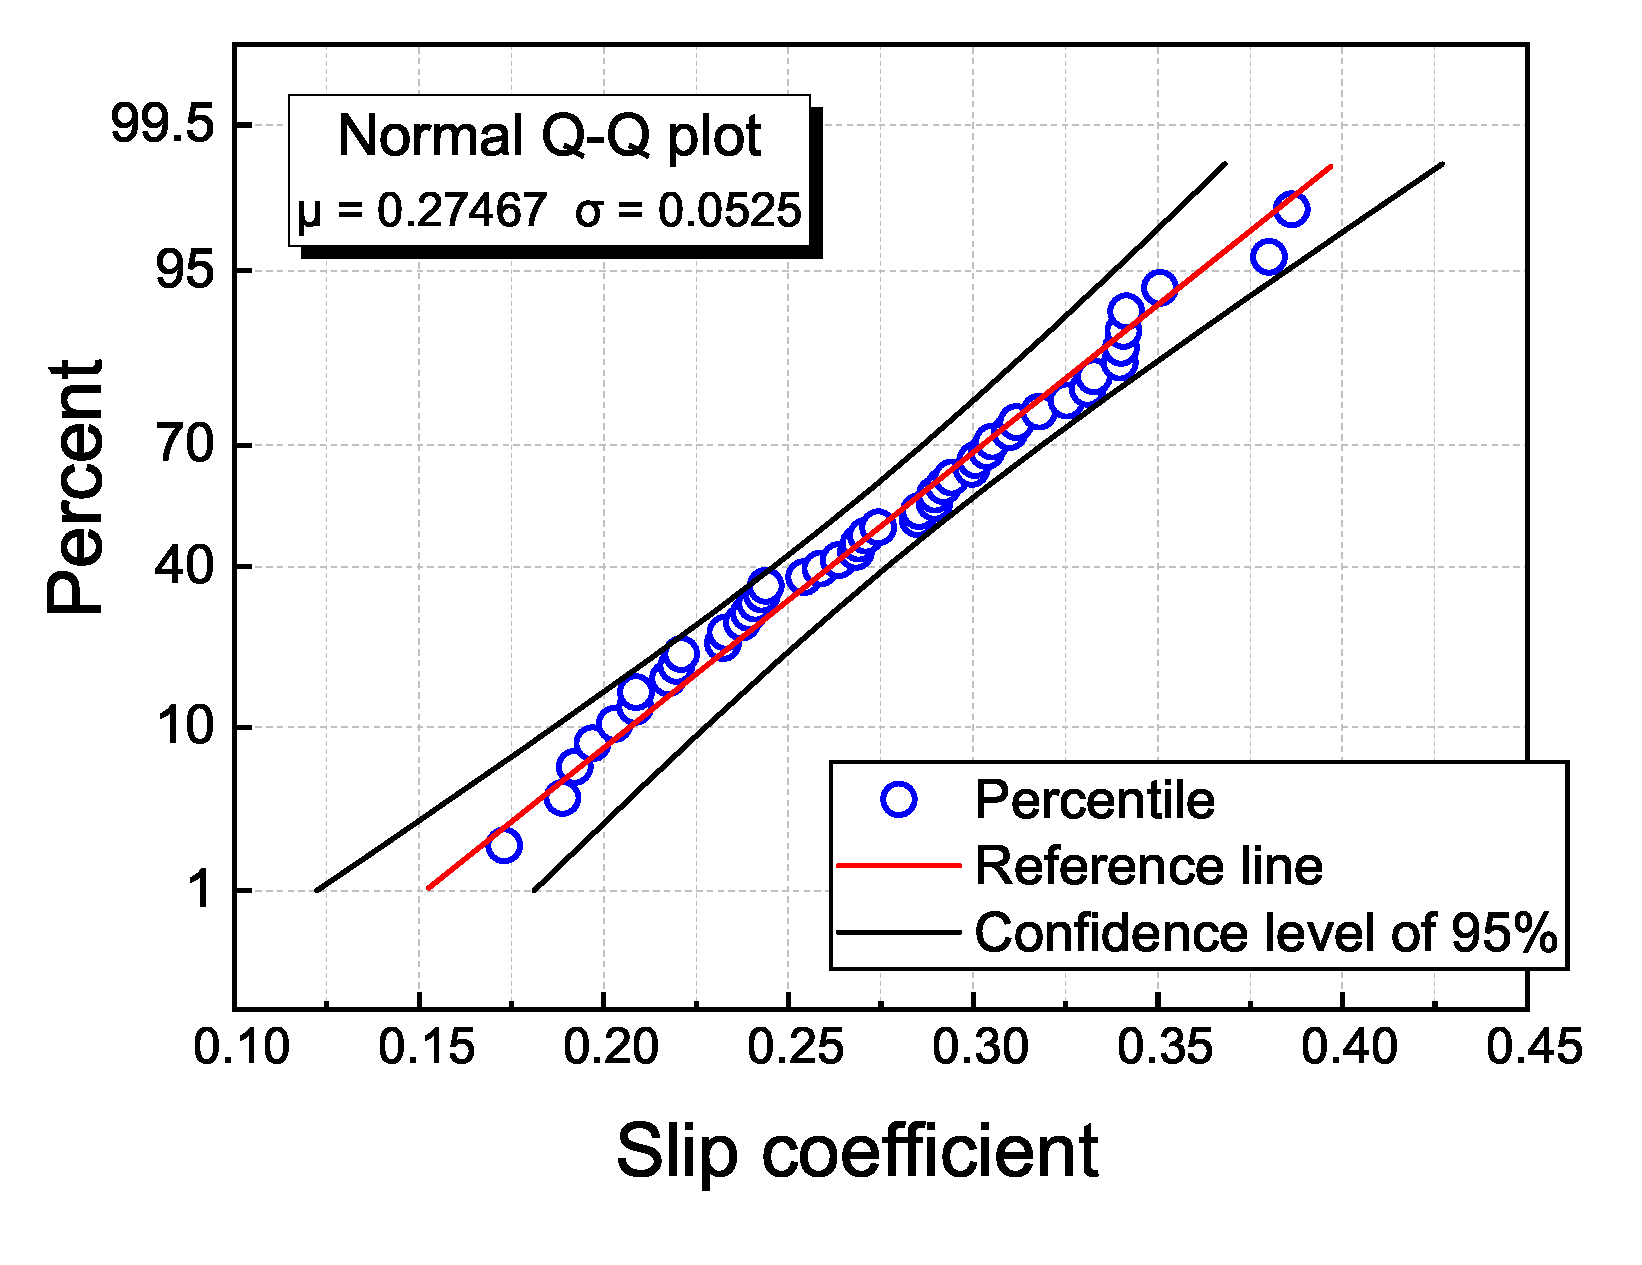
\includegraphics[width=\linewidth]{imgs/ch3/fig10b.eps}
    \caption{Q-Q plot}
    \label{ch3fig10b}  
    \end{subfigure}
    \caption{Slip coefficient distribution}
    \label{ch3fig10} 
\end{figure}

Besides, when the riveted joint surface is red lead paint, replacing the rivet with a high-strength bolt, the expected slip coefficient is 0.25-0.28 by Railway technical research institute in Japan \cite{rtri1992Manual}. However, in this experiment, it can be calculated that there is a 36\% probability that the slip coefficient is below 0.25. 

The specimens' size could cause this, and the red lead distribution is uneven, resulting in a very low slip coefficient accrued in some specimens.

The relationship between the slip coefficient and the clamping force is shown in Fig. \ref{ch3fig11}. It can be observed from the figure that the degree of dispersion of the slip coefficient has no obvious relationship with the change of clamping force; also, it can be calculated that the correlation coefficient between clamping force and slip coefficient is 0.21. On the other hand, the relationship between the slip load and clamping force is shown in Fig. \ref{ch3fig12}. As the clamping force increases, the slip load also increases.

\begin{figure}
\centering
\begin{minipage}[t]{0.48\textwidth}
\includegraphics[width=\linewidth]{imgs/ch3/fig11.eps}
\caption{The relationship between the slip coefficient and the clamping force.}
\label{ch3fig11}
\end{minipage}
\begin{minipage}[t]{0.48\textwidth}
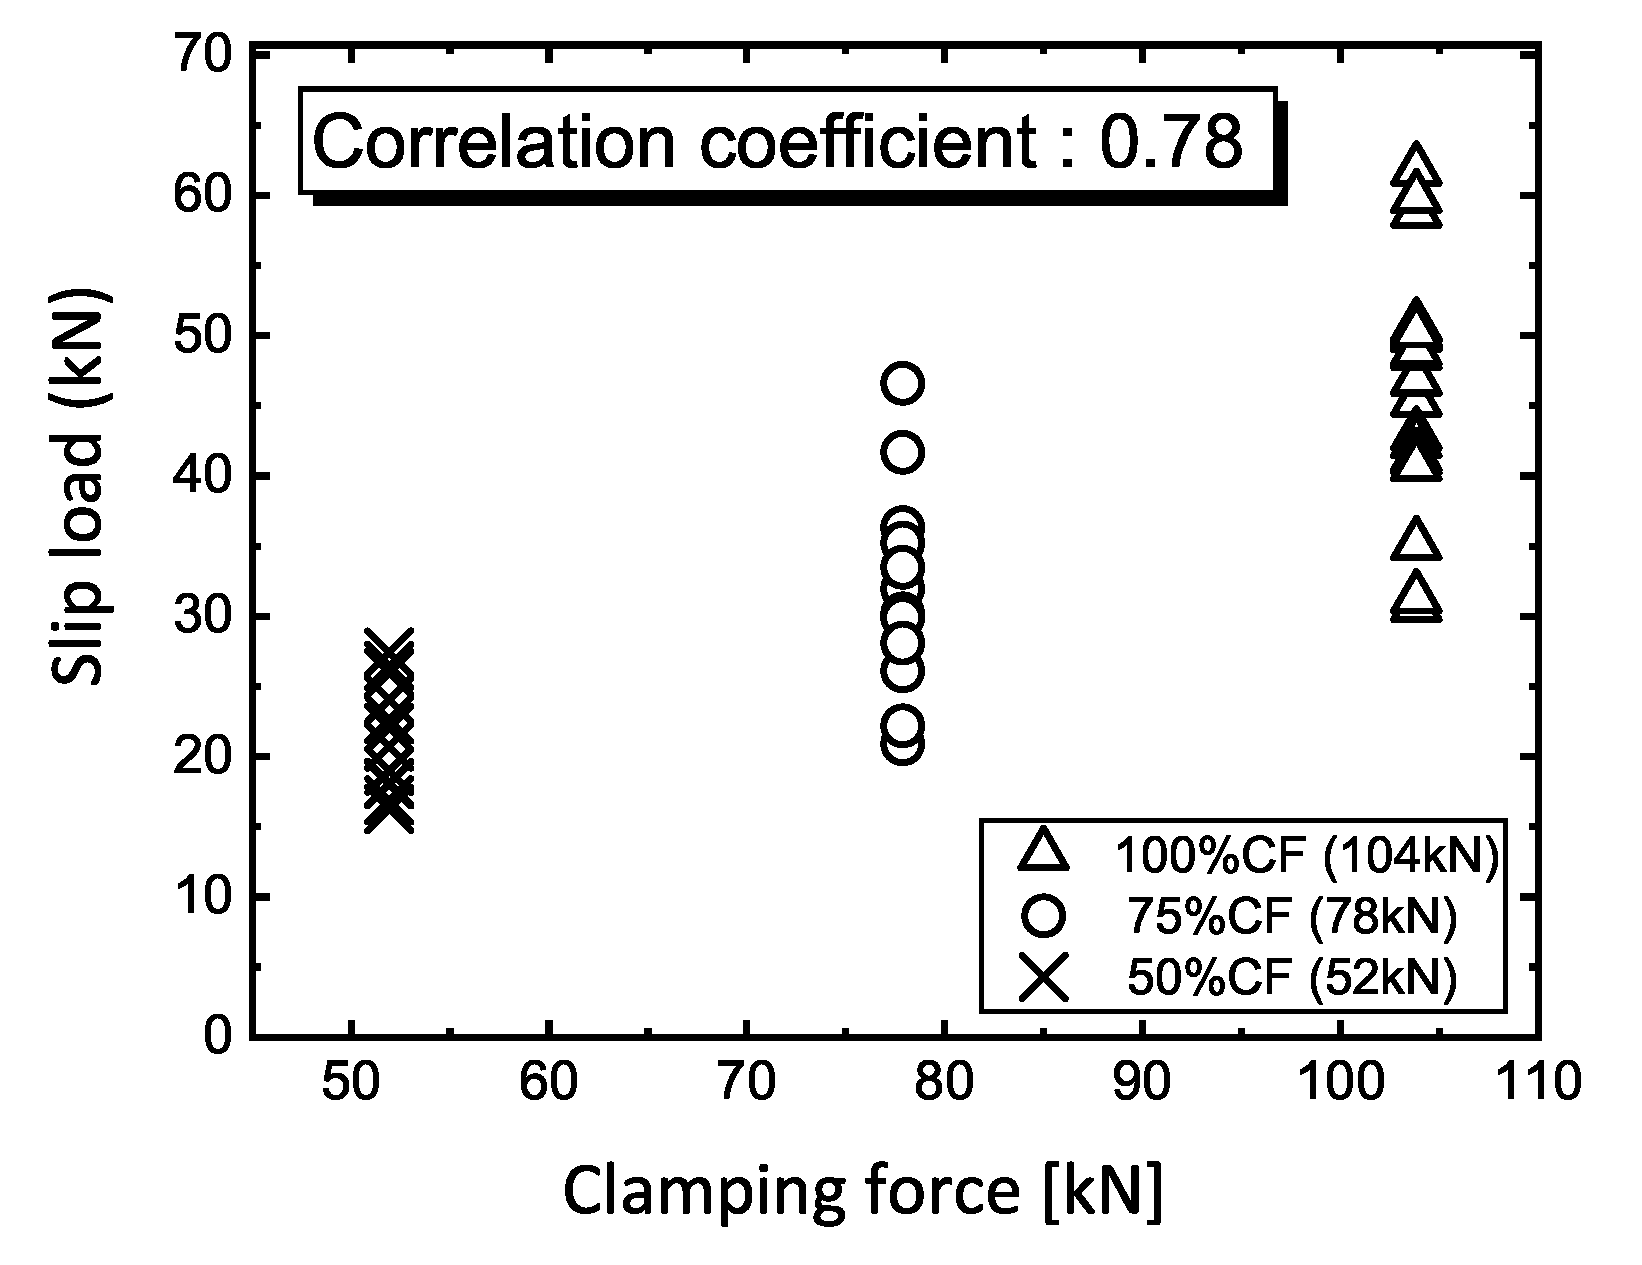
\includegraphics[width=\linewidth]{imgs/ch3/fig12.eps}
\caption{The relationship between the slip load and the clamping force.}
\label{ch3fig12}
\end{minipage}
\end{figure}

In addition, the average friction coefficient obtained is 0.295, which is 0.02 larger than the average slip coefficient of 0.274. The friction coefficient is calculated by dividing the load by the clamping force, which is taken when slippage has occurred. 

\subsection{Contact pressure distribution test}

The observation of the joint surface in section \ref{ch3sec2-1} revealed that the red lead surface distribution of specimens was much not uniform, and the red lead distribution of each specimen was also very different. In this study, a pressure distribution test is performed to investigate the influence of red lead distribution on the contact pressure and the slip coefficient. 

\subsubsection{Measuring methods}
A pressure measurement film is put into the joint surface, and then the standard clamping force is applied to the specimen by the screw-jack. When detected pressure, the film will be colored redder as the pressure increases.

\subsubsection{Measuring result}

Eight sets of specimens are conducted with a pressure distribution test. The pressure distribution was very uneven according to the aging condition of red lead paint, and the residual condition of red lead directly reflected the pressure distribution. Fig. \ref{ch3fig13} shows the pressure test results of the specimens' joint surface with a slip coefficient of 0.284 and the joint surface's condition before/after the slip test.


\begin{figure}
\includegraphics[width=\linewidth]{imgs/ch3/fig13.pdf}
\caption{Pressure contour figures and the condition before/after slip test.}
\label{ch3fig13}  
\end{figure}

As shown in Fig. \ref{ch3fig13}-b, the range marked with red is detected contact pressure area; the white areas have not detected contact pressure. The slip test assumes that the pressure is evenly distributed on the joint surface; however, the measuring results show that red lead paint's surface does not satisfy the average pressure distribution assumption.

As shown in Fig. \ref{ch3fig13}-c, after the slip test, the red lead paint on the joint surface was damaged. The traces of the slippage can be clearly seen. However, there are no traces of slippage near the marked red circle. The joint surface friction condition was very similar to the pressure distribution, as shown in Fig. \ref{ch3fig13}-b. It can be inferred that the white areas where no pressure is detected have no effective resistance to the friction and can be defined as the invalid contact area. On the contrary, the effective contact area is defined as where the contact pressure is detected. The effective contact pressure $σ_e$ is calculated by the effective contact area and clamping force.

\begin{equation}
    σ_e=N_0/S_e
\end{equation}
Where $N_0$ is clamping force;$ S_e$ is effective contact area. 

\begin{figure}
\centering
\includegraphics[width=0.65\linewidth]{imgs/ch3/fig14.pdf}
\caption{The relationship between slip coefficient and effective contact pressure}
\label{ch3fig14}  
\end{figure}

The relationship between slip coefficient and the effective contact pressure is shown in Fig. \ref{ch3fig14}. The effective contact area for each specimen is different, so although the same clamping force they have, calculated effective contact pressure is different. The correlation coefficient between the slip coefficient and the effective contact pressure is calculated as 0.476. No apparent relationship between the slip coefficient and the effective contact pressures has been observed. It could be considered that reason is the contact pressure was unevenly distributed in the effective contact area. Furthermore, the invalid pressure area and low contact pressure area do not effectively resist friction, and local slip has likely occurred. 


\subsection{Summarize for the slip coefficient}
In this study, the joint part cut out from a 90-year-old riveted bridge's cross-beam. It evaluated the riveted joint surface's aging condition with red lead by microscope observation and chemical analysis. The slip and pressure distribution tests are also conducted to investigate the joint surface's slip coefficient of the riveted joints and the pressure distribution of riveted joints' surface. 

Given the results of the present research, the obtained conclusions are as follows: 

\begin{itemize}
    \item The distribution of red lead on the joint surface is not flat, the adhesion of the red lead has deteriorated, and the black oxide on the surface of the steel can be observed. In addition to the red lead film, vinyl acetate was also discovered by the FT-IR spectra analysis. 

    \item The average slip coefficient was 0.274, and the coefficient of variation was 0.191.-2σ is 0.169. The 95\% confidence interval for the slip coefficient is 0.259-0.289. 

    \item According to the relationship between the slip coefficient and clamping force, it has been confirmed that the change of the clamping force will not affect the slip coefficient.

    \item The pressure distribution test could be concluded that due to the joint surface is not flat, the pressure distribution is also very uneven, and very high pressure is generated locally. On the contrary, there is no effective pressure applied in some places called an invalid contact area. Besides, the slip coefficient has no obvious relationship with effective contact pressures.
    
\end{itemize}

\section{Tensile test of partially replacement of riveted joint}

\subsection{Background}

The girders of steel riveted bridges are often thin plates and the same applies to the joints. For riveted joints, the joint bearing capacity is generally determined by the rivet/base plate bearing pressure or the shear of the rivet, but it may also be determined by the yielding of the base plate. This study investigates repair and reinforcement methods for riveted joints where the base plate is yield-precedent (thin plate), by replacing the rivets with high-strength bolts.

The following three methods can be used to repair rivets that have corroded due to age-related deterioration. The following three methods can be identified as methods of repairing rivets that have corroded due to age: (1) replacement with new rivets, (2) high-strength bolt support joints, and (3) replacement with high-strength bolt friction type joints. However, the application of method (1) is difficult due to the fact that few construction engineers are available. Therefore, replacement with a support high-strength bolt is the most promising method. However, the adoption of a support joint is difficult to control the hole diameter, and from the viewpoint of reliable construction on site, the most promising method is the replacement with a high-strength bolt for friction bonding. In addition, from the viewpoints of economy and workability, partial replacement is often considered preferable to total replacement. In this study, joint tensile tests are carried out to determine the load carrying capacity of existing riveted joints when partially or fully replaced with high-strength bolts for friction joints, and the slip coefficient that can be expected in the design.


\subsection{Specimens of test}

In this study, joints part on the crossbeam(two-sided riveted joints) were sampled from the Dojima Bridge. The sampling locations and cut-off position are shown in Fig. \ref{fig-cutoff}.

\begin{figure}
    \centering
    \includegraphics[width=0.6\textwidth]{imgs/ch4/figA1.pdf}
    \caption{Cut off position of each specimens}
    \label{fig-cutoff}
\end{figure}

The specimen case is shown in Fig. 3.2. The tests were carried out using a riveted joint consisting of a total of five rivets (Specimen 1) in one row and three columns on each side as the basic case and replacing all rivets with high-strength bolts for friction joints (Specimen 2) and partially replacing rivets with high-strength bolts because in actual repair design and repair work, only corroded or fallen out rivets may be replaced with high-strength bolts. The case where rivets are partially replaced with high-strength bolts (specimens 3, 4 and 5) is examined, as in actual repair design and repair work, only rivets that have corroded or fallen out may be replaced with high-strength bolts.

\begin{figure}
    \centering
    \includegraphics[width=0.8\textwidth]{imgs/ch3/riveexpcase.pdf}
    \caption{Experiment case}
    \label{fig:enter-label}
\end{figure}

% Prior to the tests, specimens cut in the direction of the shaft centre were fabricated as shown in Fig. 3.3, the hole diameter and the gap between the rivet and the steel plate were measured and the filling status of the rivets was observed in order to ascertain the filling status of the rivets. If gaps existed, water flowed through the gaps and corrosion damage was also observed.